%!TEX root = ../problems.tex
\begin{figure}[h!]
\centering
\begin{minipage}{0.4\textwidth}
\centering
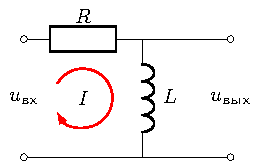
\includegraphics[width=\linewidth]{chem/task3}
\caption{$RL$--контур}
\label{fig:2figsA}
\end{minipage}
\qquad
\begin{minipage}{0.4\textwidth}
\centering
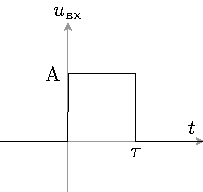
\includegraphics[width=\linewidth]{ris/task2_input}
\caption{Входное напряжение}
\label{fig:2figsB}
\end{minipage}
\end{figure}
\begin{task}
	Определите отклик $u_\out(t)$ $RL$-цепи, изображенной на рисунке, на воздействие единичного импульса длительностью $\tau$. 
	Нарисуйте график отклика. 
	Какова переходная характеристика цепи? 
	При выполнении какого условия будет осуществляться приближённое дифференцирование входной цепи?
	Решить задачу с ненулевыми начальными условиями.
\end{task}
\begin{proof}[\rm{\textbf{Решение}}]
Найдем образ входного импульса преобразованием Лапласа: 
\begin{equation}
	u_\in(t)=E\cdot\H(t)-E\cdot\H(t-\tau)
	\quad\Rightarrow\quad
	u_\in(t)\LT \frac{E}{p}-\frac{E}{p}e^{-p\tau}=
	\frac{E}{p}\qty(1-e^{-p\tau})
\end{equation}
Надо учесть, что в контуре могут быть заданы начальные условия - ток $i_0$.
Тогда начальное напряжение на катушке $u_L(0)=i_0\cdot pL$, а его образ $u_L(0) \LT \frac{i_0 pL}{p}=i_0L$. 
Это напряжение можно трактовать как часть ЭДС.

Обозначим суммарный ток в контуре за $I(p)$. Тогда, так как сумма падений напряжения на каждом элементе равна нулю, получим следующее выражение:
\begin{equation}
	\frac{E}{p}\qty(1-e^{-p\tau})+i_0L=(R+pL)I(p)
\end{equation}
Откуда выразим ток $I$:
\begin{equation}
	I(p)=\frac{\frac{E}{p}\qty(1-e^{-p\tau})+i_0L}{R+pL}
\end{equation}
С другой стороны, $u_\in=u_C+u_R$, а $u_C\equiv u_\out$, тогда
\begin{gather}
	u_\out(p)=u_\in(p)-u_R(p)=u_\in(p)-I(p)R=\\=
	u_\in(p)-\frac{E(1-e^{-p\tau})R}{p(R+pL)}+\frac{i_0LR}{R+pL}=
	u_\in(p)-\frac{ER}{p(R+pL)}+\frac{ERe^{-p\tau}}{p(R+pL)}-\frac{i_0LR}{R+pL}=\\=
	u_\in(p)-\frac{E\frac{R}{L}}{p(p+\frac{R}{L})}+\frac{E\frac{R}{L}e^{-p\tau}}{p(p+\frac{R}{L})}-\frac{i_0R}{p+\frac{R}{L}}
\end{gather}
Используем свойства преобразования Лапласа:
\begin{gather}
	\frac{\alpha}{p(p+\alpha)}\LT (1-e^{-\alpha t})\H(t)\\
	\frac{1}{(p+\alpha)}\LT e^{-\alpha t}\H(t)\\
	e^{{-p\tau}}F(p) \LT f(t-\tau)\H(t-\tau), \qq{где} F(p) \LT f(t)
\end{gather}
Учтя, что $u_\in(p) \LT u_\in(t)$, произведем преобразование:
\begin{gather}
	u_\out(t)=u_\in(t)-E(1-e^{-\frac{R}{L} t})\H(t)+E(1-e^{-\frac{R}{L} (t-\tau)})\H(t-\tau)-i_0Re^{-\frac{R}{L} t}\H(t)=\\=
	\cancel{E\cdot\H(t)}-\cancel{E\cdot\H(t-\tau)}-E(\cancel{1}-e^{-\frac{R}{L} t})\H(t)+E(\cancel{1}-e^{-\frac{R}{L} (t-\tau)})\H(t-\tau)-i_0Re^{-\frac{R}{L} t}\H(t)=\\=\qty(E-i_0R)e^{-\frac{R}{L} t}\H(t)-Ee^{-\frac{R}{L}(t-\tau)}\H(t-\tau)
\end{gather}
Окончательно получили ответ: при воздействии прямоугольным импульсом $u_\in(t)$ амплитуды $E$ и длительностью $\tau$, на выходе получаем
\begin{equation}
 	u_\out(t)= \qty(E-i_0R)e^{-\frac{R}{L} t}\H(t)-Ee^{-\frac{R}{L}(t-\tau)}\H(t-\tau)
\end{equation} 
\paragraph{Условие дифференцирования.} 
Как нетрудно догадаться,
\begin{equation}
	u_\in=u_L+u_R=L\dv{I}{t}+IR
\end{equation}
Продифференцируем это выражение:
\begin{equation}
	\dv{u_\in}{t}=\underbrace{L\dv[2]{I}{t}}_{\dv{u_L}{t}}+\frac{R}{L}\underbrace{L\dv{I}{t}}_{u_L\equiv u_\out}
\end{equation}
Если будет выполнено условие
\begin{equation}
	\abs{\dv{u_L}{t}} \ll \abs{\frac{R}{L} u_L}
\end{equation}
Тогда будет видно, что цепочка осуществляет дифференцирование:
\begin{equation}
	u_\out=\tau_\text{цепи}\dv{u_\in}{t}
\end{equation}
где $\tau_\text{цепи}=\frac{L}{R}$.

Выясним смысл неравенства модулей на примере гармонических сигналов. Пусть входное напряжение гармоническое $u_\in=u_0e^{j\omega t}$. Тогда ток в контуре: $I=I_0e^{j\omega t}$, где $I_0=\frac{u_0}{j\omega L+R}$, и неравенство можно переписать (учтем, что $u_L=I\cdot j\omega L=I_0 j\omega L e^{j\omega t}$):
\begin{equation}
	\abs{I_0\cdot j\omega L\cdot j\omega\cdot e^{j\omega t}}\ll
		\abs{\frac{1}{\tau_\text{цепи}}I_0 \cdot j\omega L\cdot e^{j\omega t}}
	\quad \Rightarrow \quad
	\omega \ll {\frac{1}{\tau_\text{цепи}}}
	\quad \Rightarrow \quad
	T \gg \tau_\text{цепи}
\end{equation}
Таким образом, дифференцирование сигнала <<чистое>> для таких частот, период которых много больше постоянной времени цепи. Отсюда следует <<вилка выбора>> дифференцирующей цепочки: если мы будем расширять частотный диапазон <<чистого>> дифференцирования уменьшением постоянной времени, то амплитуда на выходе цепочки будет падать, и наоборот.
\end{proof}